\documentclass[12pt,a4paper]{article}
\usepackage{geometry}
\geometry{left=2.5cm,right=2.5cm,top=2.0cm,bottom=2.5cm}
\usepackage[english]{babel}
\usepackage{amsmath,amsthm}
\usepackage{amsfonts}
\usepackage[longend,ruled,linesnumbered]{algorithm2e}
\usepackage{fancyhdr}
\usepackage{ctex}
\usepackage{array}
\usepackage{listings}
\usepackage{color}
\usepackage{graphicx}
\usepackage{amssymb}
\newtheorem{theorem}{定理}
\newtheorem{lemma}[theorem]{引理}
\newtheorem{corollary}[theorem]{推论}

\begin{document}
	
	\noindent
	
	\section*{2024有限元期末考试(120分钟半开卷)}	
	
	\begin{enumerate}
		
		\item (12分)
		\begin{enumerate}
			\item 对于椭圆形方程的齐次边值问题
			
			$$\begin{cases}
				- \Delta u + q(x)u(x) = f(x), x \in \Omega \\
				u(x)\mid_{\Gamma_1} = 0,\\
				\nabla u \cdot n \mid_{\Gamma_2} = 0
			\end{cases}$$
			
			其中$\Omega$为$\mathbb{R}^2$中具有光滑边界的有界区域,$q(x) \geq 0$,$f(x)$足够光滑，边界$\partial \Omega = \Gamma_1 \ \cup \Gamma_2$且$\Gamma_1\cap\Gamma_2 = \emptyset$,试建立该边值问题的变分问题。
			
			\item 引入变量 $\boldsymbol{w} = \nabla u$,	试建立(a)的混合变分问题。		
		\end{enumerate}
		
		\item (13分)
		\begin{enumerate}
			\item 叙述并证明Lax-Milgram定理。
			\item 利用Lax-Milgram定理说明1(a)中变分问题解的存在唯一性。
		\end{enumerate}
		
		\item (10分)
		
		证明有界区域$\Omega$上的Poincaré不等式
		
		$$\|v\|_{1,\Omega} \leq C\left(|v|_{1,\Omega}+\|v\|_{0,\partial \Omega}\right), \quad \forall v \in H^1(\Omega).$$
		
		\item (15分)考虑二维空间中Hermite元的如下结果。
		\begin{enumerate}
			\item 给出三角形K上Hermite元的有限元定义。
			\item 给定区域$\Omega = (0,1) \times (0,1)$,试给出在如下网格上$\mathcal{T}_h$的$H^1(\Omega)$协调有限元空间$V_h$的定义。当$\mathcal{T}_h$如下图所示时，试着给出$V_h$的维数。
			\begin{figure}[h]
				\centering
				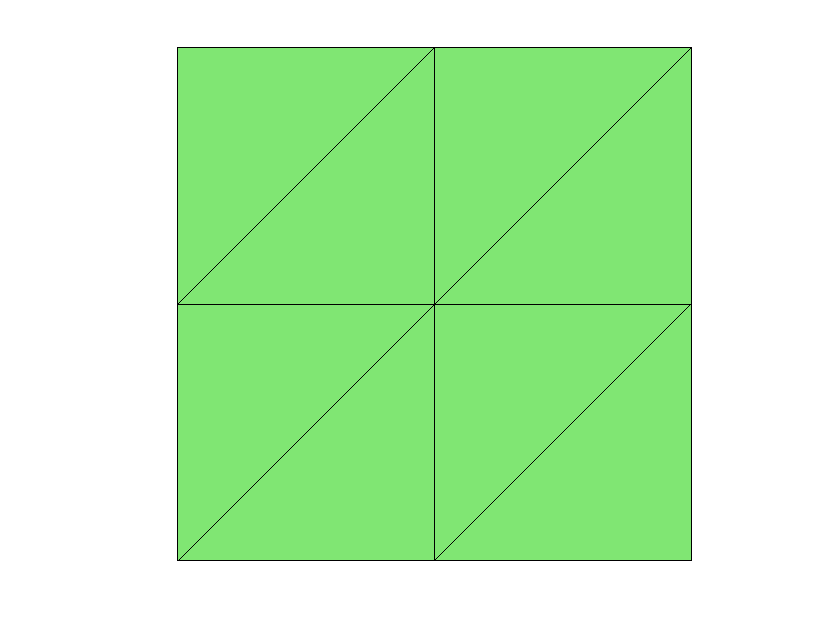
\includegraphics[width=0.5\linewidth]{mesh.png}
				\label{fig:mesh}
			\end{figure}
			
			\item 给定三角形$K$及其直径$h_K$,假设$u \in H^4(K)$,写出插值算子的定义，并且给出$\|u-\Pi_K u\|_{0,K}$和$\|u-\Pi_K u\|_{1,K}$的插值误差估计结果(不用证明)。
		\end{enumerate}
		
		

		\item (10分) 给定三角形$K$及其直径$h_K$
		\begin{enumerate}
			\item 设$e$是$K$的一条边，利用参考单元上$\widehat{K}$上$\|v\|_{0,\partial \widehat{K}} \leq C\|v\|_{1,\widehat{K}}$证明
			
			$$|e|^{-\frac{1}{2}} \|v\|_{0,e} \leq C\left(h_K^{-1}\|v\|_{0,K}+|v|_{1,K}\right), \forall v \in H^1(K).$$
			
			\item 证明逆估计
			
			$$\|v\|_{2,K} \leq Ch_K^{-2}\|v\|_{0,K}, \forall v \in P_2(K).$$
		\end{enumerate}
		
		\item (20分) 假设$\Omega$是$\mathbb{R}^2$中有界凸区域。$u \in H^3(\Omega) \cap H_0^1(\Omega)$满足Poisson问题
		
		$$\begin{cases}
			- \Delta u = f, in \Omega \\
			u\mid_{\partial \Omega} = 0, 
		\end{cases}$$ 
		
		$u_h \in V_{h0}$是Lagrange二次元的有限元解。
			
		\begin{enumerate}
			\item 请写出变分问题和离散问题
			\item 写出Lagrange二次元在单元$K$上的基函数。
			\item 试证明$L^2$范数下的误差估计
			$$\|u-u_h\|_{0,\Omega} \leq Ch^3|u|_{3,\Omega}.$$
		\end{enumerate}	
		
		\item (20分) 考虑凸区域$\Omega$上的Stokes问题的混合变分形式
		
		$$\begin{cases}
			- \Delta \boldsymbol{u}+\nabla p = \boldsymbol{f},\quad in \ \Omega \\
			\mathrm{div} \boldsymbol{u} = 0,\quad in \ \Omega \\
			u\mid_{\partial \Omega} = 0.
		\end{cases}$$
		
		\begin{enumerate}
			\item 写出Stokes问题的混合变分形式。
			\item 写出Stokes问题基于$P_2-P_0$元的离散方法。
			\item 写出连续和离散inf-sup条件，并构造一个插值$\Pi_h:(H_0^1(\Omega)^2) \rightarrow V_h$满足如下的Fortin准则并给出证明
			
			$$b(\boldsymbol{v}-\Pi_h \boldsymbol{v},q_h),\quad q_h \in Q_h$$
			$$\|\Pi_h \boldsymbol{v}\|_{1,\Omega} \leq C\|\boldsymbol{v}\|_{1,\Omega}, \quad \boldsymbol{v} \in (H_0^1(\Omega)^2)$$
		\end{enumerate}
	\end{enumerate}
	

\end{document}

